\documentclass[a0paper,portrait]{baposter}

\usepackage[utf8]{inputenc}

\usepackage{amsmath}    
\usepackage{amsfonts}   
\usepackage{amsthm} 
\usepackage{caption}
\usepackage{graphicx}
\usepackage{paralist}
\usepackage{xcolor}

\definecolor{darktyrkis}{RGB}{0,143,149}

\begin{document}
\begin{poster}{
  columns=2,
	grid=false,
	borderColor=darktyrkis,
	headerColorOne=darktyrkis,
	headerColorTwo=darktyrkis,
	headerFontColor=white,
  headerheight=8em,
	boxColorOne=white,
  boxpadding=1em,
	headershape=rounded,
	headerfont=\Large\textsf,
	textborder=rounded,
	background=shadetb,
  bgColorOne=darktyrkis!10,
  bgColorTwo=darktyrkis!30,
	headerborder=open,
  boxshade=plain,
  eyecatcher=false
}
%%% Eye Catcher %%%%%%%%%%%%%%%%%%%%%%%%%%%%%%%%%%%%%%%%%%%%%%%%%%%%%%%%%%%%%%%
{
}
%%% Title %%%%%%%%%%%%%%%%%%%%%%%%%%%%%%%%%%%%%%%%%%%%%%%%%%%%%%%%%%%%%%%%%%%%%
{ \Huge Evolutionary optimization of machine learning pipelines}
%%% Authors %%%%%%%%%%%%%%%%%%%%%%%%%%%%%%%%%%%%%%%%%%%%%%%%%%%%%%%%%%%%%%%%%%%
{
  %\vspace{1em}
  \\Gabriela Suchopárová
}
%%% Logo %%%%%%%%%%%%%%%%%%%%%%%%%%%%%%%%%%%%%%%%%%%%%%%%%%%%%%%%%%%%%%%%%%%%%%
{
}

\small

%%% Abstract %%%%%%%%%%%%%%%%%%%%%%%%%%%%%%%%%%%%%%%%%%%%%%%%%%%%%%%%%%%%%%%%%%
\headerbox{Abstract}{name=abstract,column=0,row=0,span=2}{
The subject of this work is the automated machine learning (AutoML), which
is a field that aims to automatize the process of model selection for a given machine
learning problem. We have developed a system that, for a given supervised
learning task represented by a dataset, finds a suitable pipeline --- combination
of machine learning, ensembles and preprocessing methods. For the search we
designed a special instance of the developmental genetic programming which enables
us to encode directed acyclic graph pipelines into a tree representation.
The system is implemented in the Python programming language and operates
on top of the scikit-learn library. The performance of our solution was tested on
72 datasets of the OpenML-CC18 benchmark with very good results.
}


% last box to reference
\headerbox{OpenML-CC18}{name=box3,column=0,span=2,above=bottom}{
% TODO popisek???
Here will be a nice description of the experiment. May be reduced to only one of the
graphs for illustrative purpose only.

\vspace{0.5em}
\begin{minipage}{.5\textwidth}
  \centering
  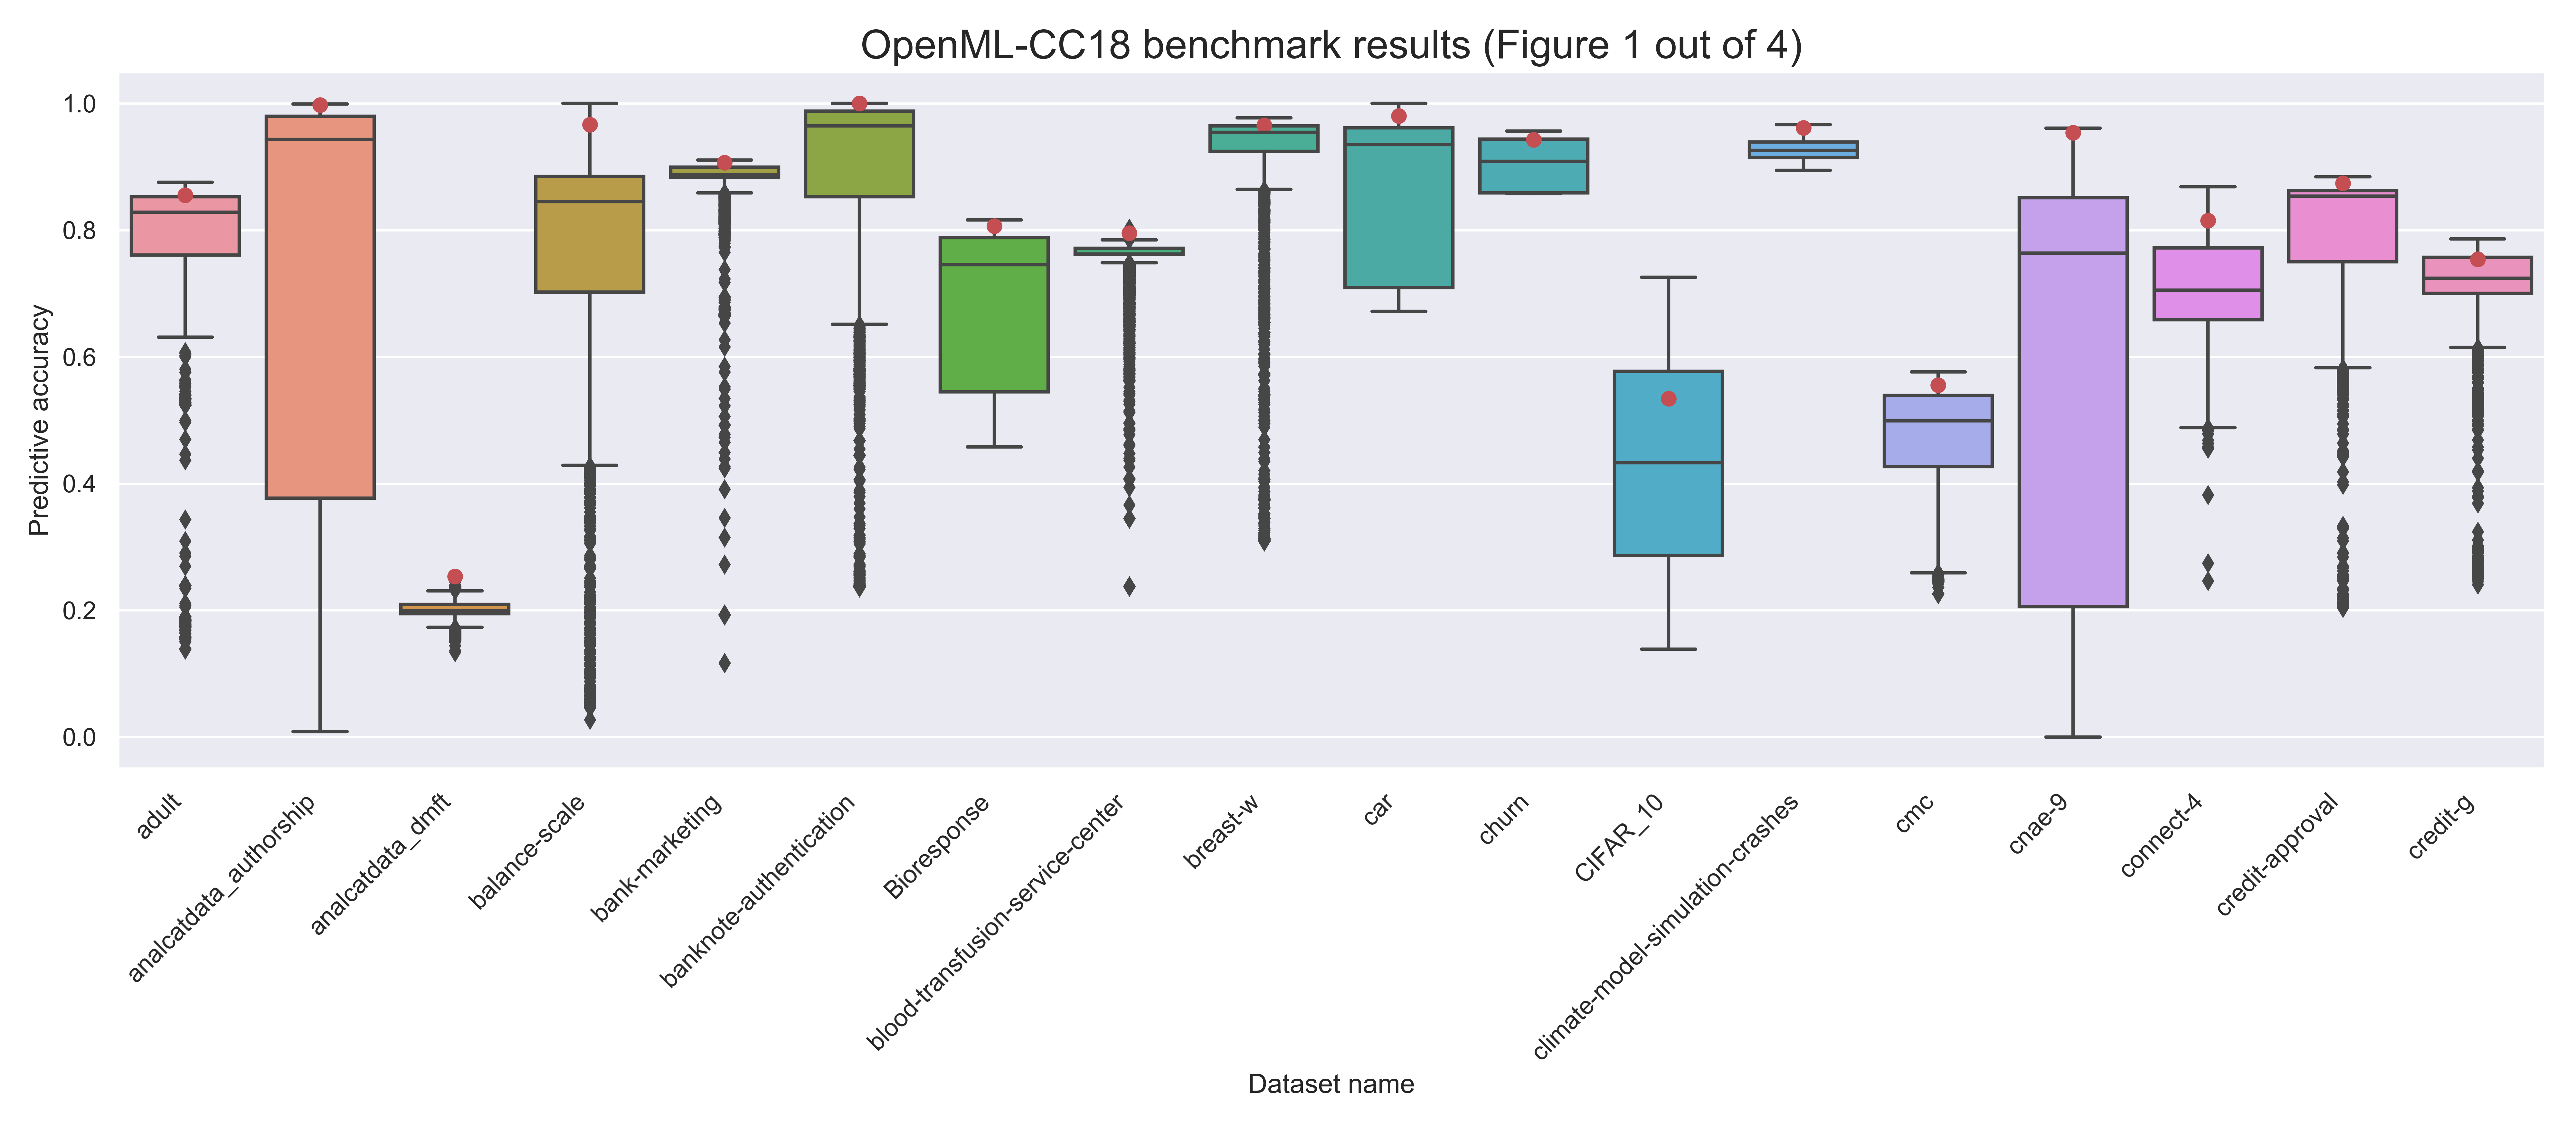
\includegraphics[width=0.9\linewidth]{../img/openml-boxplot0-hdpi.png}

\end{minipage}%
\begin{minipage}{.5\textwidth}
  \centering
  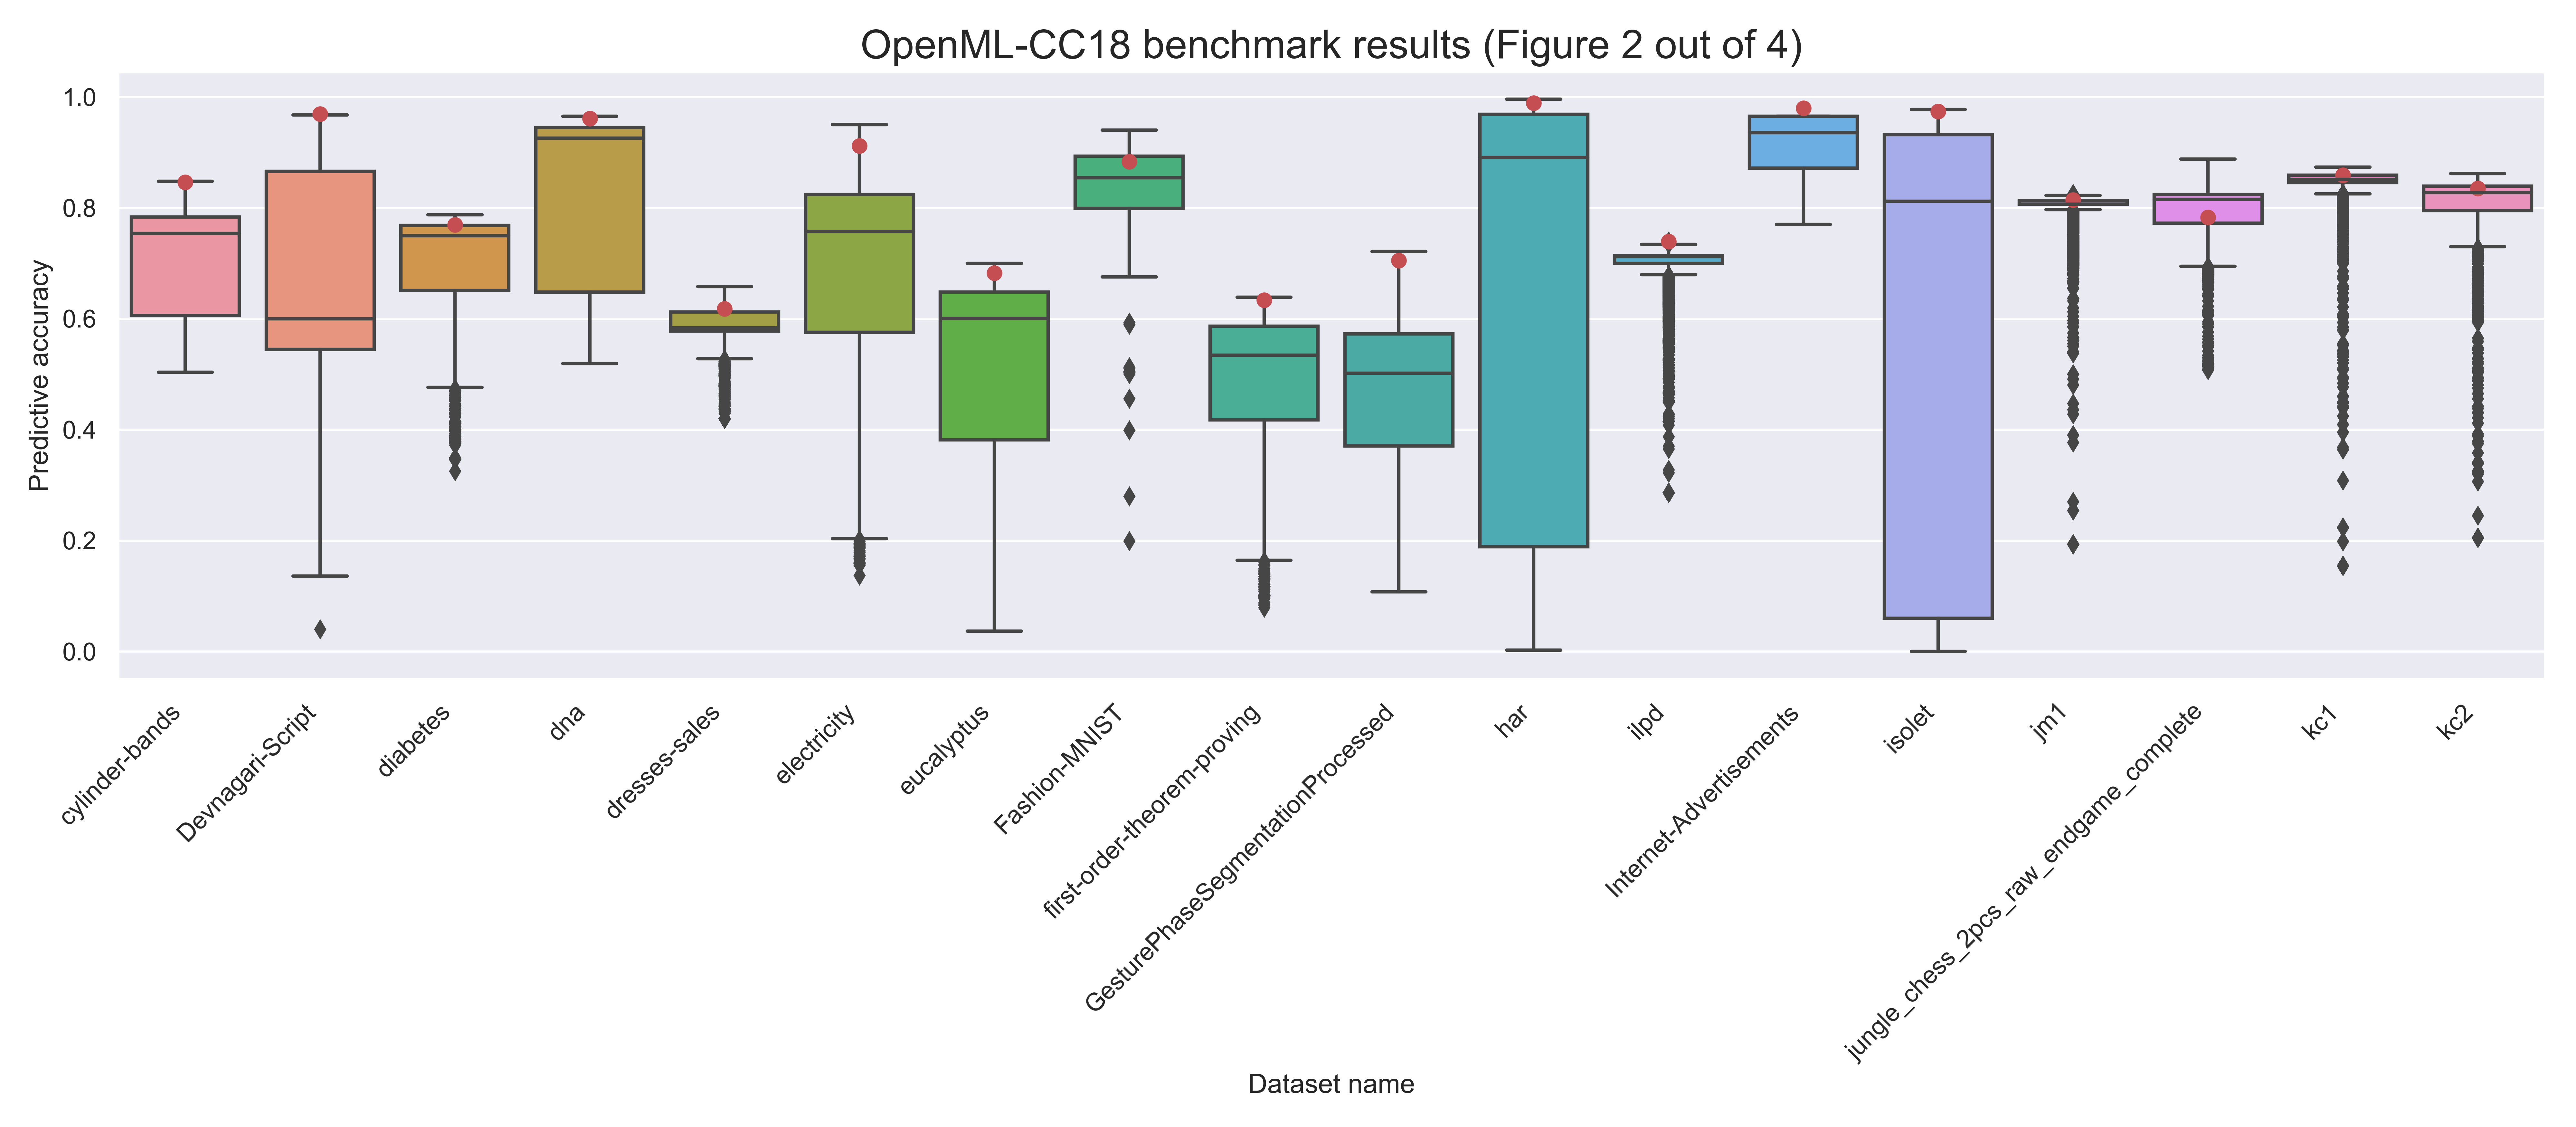
\includegraphics[width=0.9\linewidth]{../img/openml-boxplot1-hdpi.png}

\end{minipage}

\vspace{0.5em}

\begin{minipage}{.5\textwidth}
  \centering
  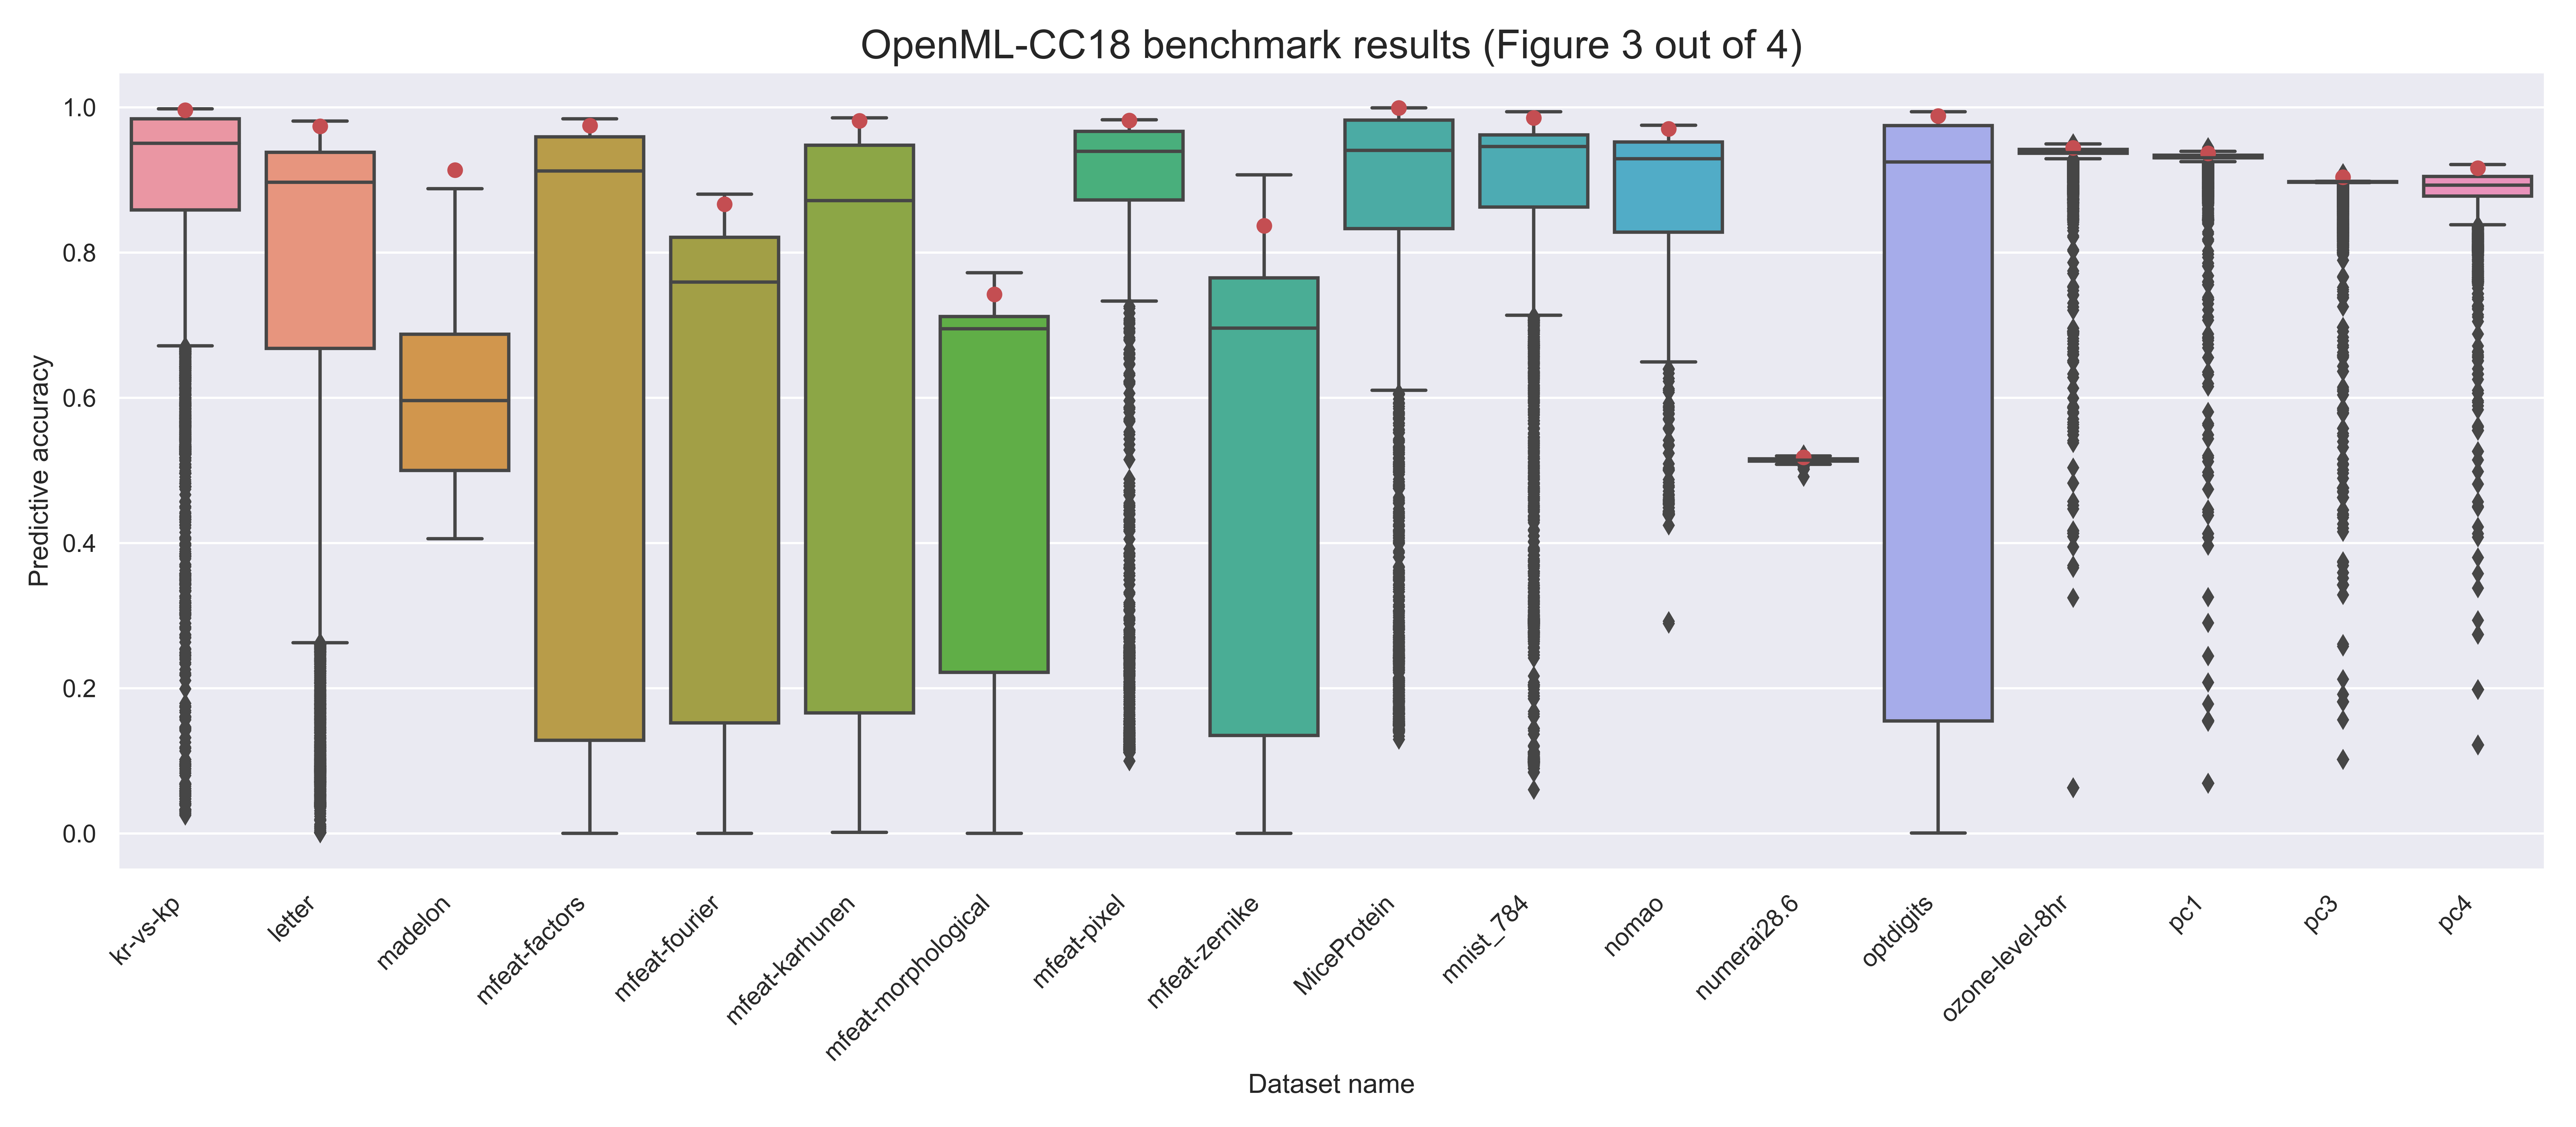
\includegraphics[width=0.9\linewidth]{../img/openml-boxplot2-hdpi.png}

\end{minipage}%
\begin{minipage}{.5\textwidth}
  \centering
  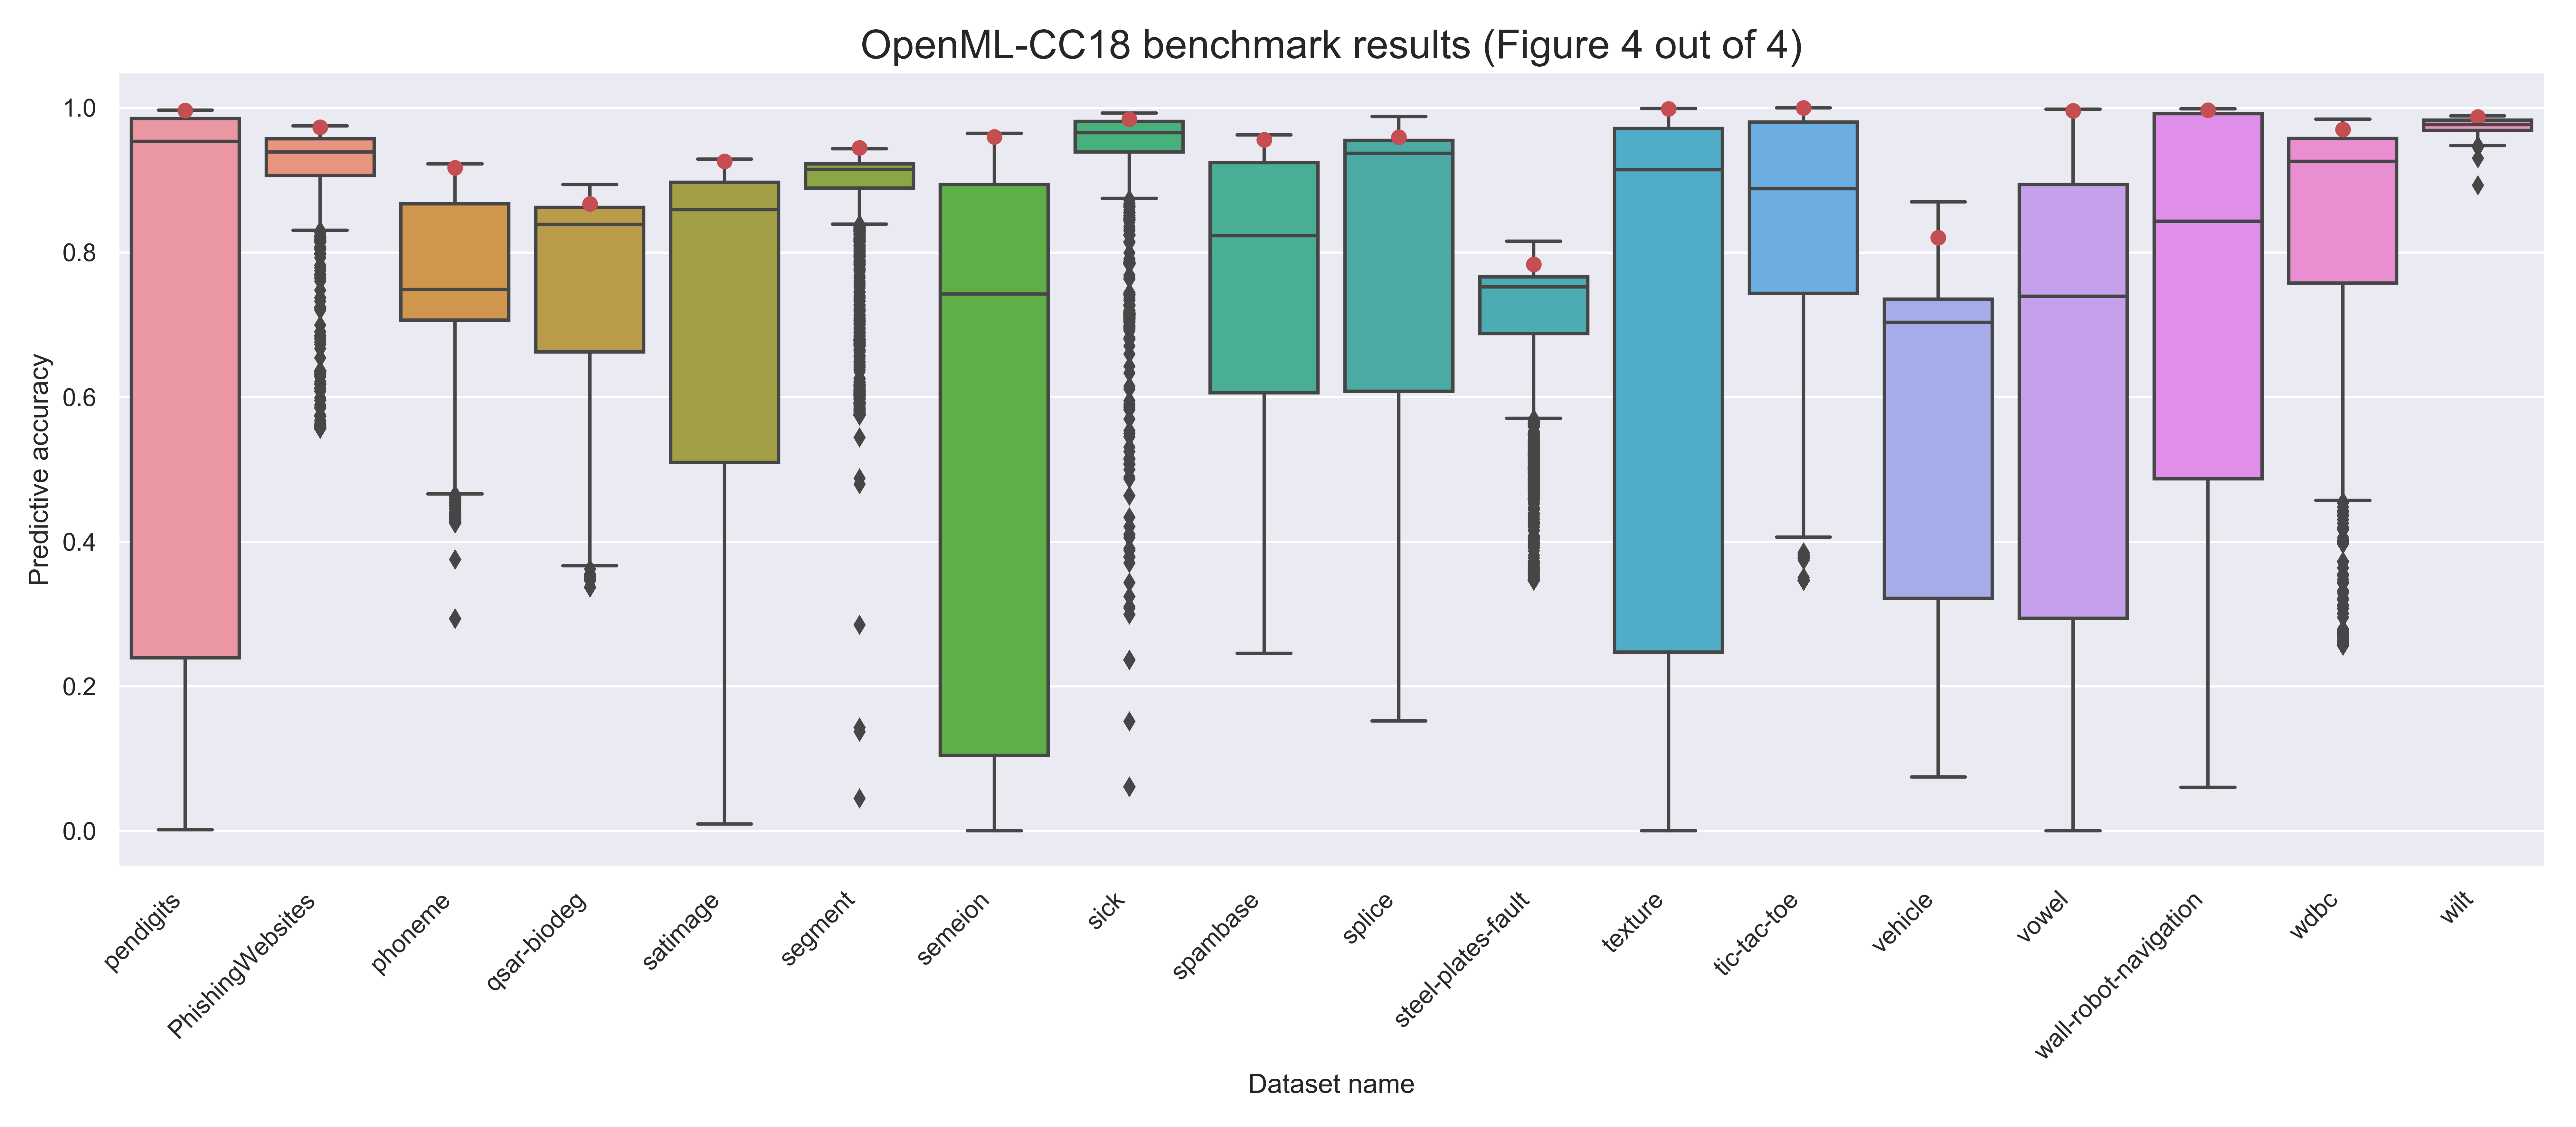
\includegraphics[width=0.9\linewidth]{../img/openml-boxplot3-hdpi.png}

\end{minipage}
}

%%% Box 1 %%%%%%%%%%%%%%%%%%%%%%%%%%%%%%%%%%%%%%%%%%%%%%%%%%%%%%%%%%%%%%%%%%%%%
\headerbox{Workflows}{name=box1,column=0,below=abstract, above=box3}{
Here will be a general workflow description.

\begin{minipage}{\textwidth}
  \centering
  \vspace{0.5em}
  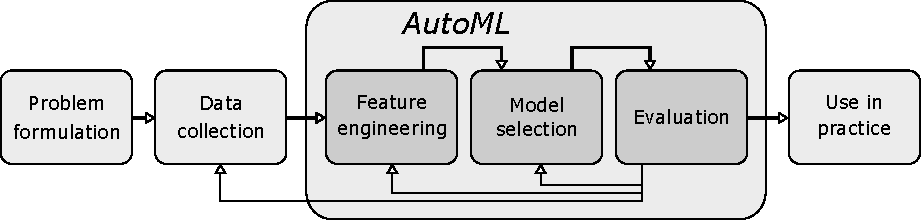
\includegraphics[width=0.7\linewidth]{../img/workflow-pdfa.pdf}
  \vspace{0.5em}
\end{minipage}

Existing systems focused only on\ldots The subject of this type of AutoML are mainly
pipelines. Represented by a DAG.

\begin{minipage}{\textwidth}
  \centering
  \vspace{0.5em}
  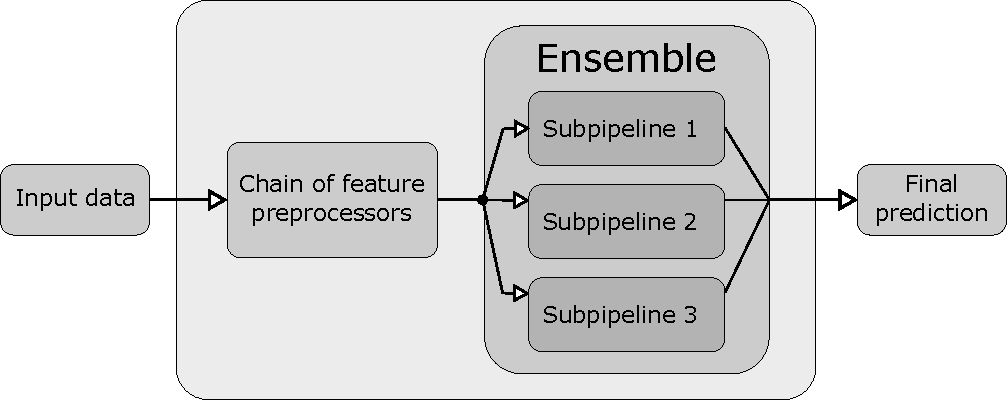
\includegraphics[width=0.7\linewidth]{../img/pipeline-pdfa.pdf}
  \vspace{0.5em}
\end{minipage}
}

%%% Box 2 %%%%%%%%%%%%%%%%%%%%%%%%%%%%%%%%%%%%%%%%%%%%%%%%%%%%%%%%%%%%%%%%%%%%%
\headerbox{Developmental GP}{name=box2,column=1,below=abstract,above=box3}{
For pipeline optimization, we used the genetic programming (GP), which is a subfield
of evolutionary algorithms. An individual in GP is in fact a computer program. Usually,
it is represented as an expression tree. The fitness of the tree is determined by
running the program, or also evaluating all functions and their arguments.

\vspace{0.5em}
\begin{minipage}{\textwidth}

  \begin{minipage}{.5\textwidth}
    \centering
    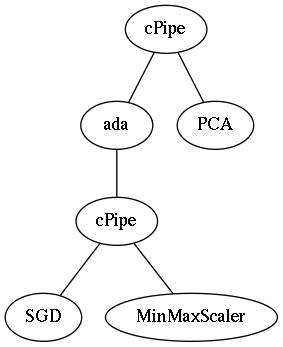
\includegraphics[width=0.45\linewidth]{../img/ada.png}

  \end{minipage}%
  \begin{minipage}{.5\textwidth}
    \centering
    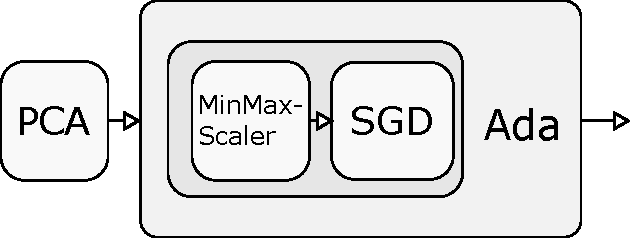
\includegraphics[width=0.8\linewidth]{../img/ada-pdfa.pdf}
  \end{minipage}
  
  \captionof{figure}{Example of an encoded pipeline}
  \label{fig:encoding}
\end{minipage}
\vspace{0.5em}

We created a specific encoding that enables to convert pipelines in the form of a DAG into
a tree representation. Instead of directly encoding pipeline steps as nodes, we apply the
developmental GP, where the nodes represent \emph{operations} that create the pipeline.

An example of the encoding is shown in Figure \ref{fig:encoding}. The tree individual
contains instructions which construct the actual pipeline:

\vspace{0.5em}
\textbf{cPipe} --- create a pipeline with a preprocessor chain and an estimator
\begin{compactitem}
  \item[-] \textbf{ada} --- insert an AdaBoost ensemble with a base-estimator
  \begin{compactitem}
    \item[-] \textbf{cPipe} --- create a pipeline with a preprocessor chain
    \begin{compactitem}
      \item[-] \textbf{SGD} --- insert a SGD classifier
      \item[-] \textbf{MinMaxScaler} --- insert a MinMaxScaler
    \end{compactitem}
  
  \end{compactitem}
  
  \item[-] \textbf{PCA} --- insert the PCA preprocessor
\end{compactitem}
}

\end{poster}

\end{document}